%HW02.tex
%Second Homework -- Math 221H
%
%  The percent sign is a comment character
%
%%%%%%%%%%%%%%%%%%%%%%%%%%%%%%%%%%%%%%%%%%%%%%%%%%%%%%%%%%%%%%%%%%%%%%%%%%%%%%%%%%
%
%   Look these up on line.  The first sets the type of document, and the next are for mathematics symbols, graphics and color
%
\documentclass[12pt]{article}
\usepackage{amssymb,amsmath}
\usepackage{graphicx}
\usepackage[usenames,dvipsnames,svgnames,table]{xcolor}
\usepackage{multirow}   % This is for more control over tables
%%%%%%%%%%%%%%%%%%%%%%%%%%%%%%%%  Layout     %%%%%%%%%%%%%%%%%%%%%%%%%%%%%%%%%%%%%%
\usepackage{vmargin}
\setpapersize{USletter}
\setmargrb{2cm}{1cm}{2cm}{1cm} % --- sets all four margins LTRB


\newcommand{\RR}{{\mathbb R}}  % This is the backboard bold symbol for the real numbers.  Note how it is used below
\newcommand{\NN}{{\mathbb N}}  % 
\newcommand{\ZZ}{{\mathbb Z}}  %

\newcommand{\calP}{{\mathcal P}}  %Caligraphic P for power set

\newcommand{\bfa}{{\bf a}}    %Vectors
\newcommand{\bfb}{{\bf b}}    %Vectors
\newcommand{\bfc}{{\bf c}}    %Vectors
\newcommand{\bfd}{{\bf d}}    %Vectors
\newcommand{\bfv}{{\bf v}}    %Vectors
\newcommand{\bfi}{{\bf i}}    %Unit Vectors
\newcommand{\bfj}{{\bf j}}    %Unit Vectors
\newcommand{\bfk}{{\bf k}}    %Unit Vectors

\newcommand{\sep}{{\ :\ }}     % This is for the : in our notation for building sets.
                               % an acceptable (and common) alternative is \mid  (try it!)

%%%%%%%%%%%%%%%%%%%%%%%%%%%%%%%%%%%%%%%%%%%%%%%%%%%%%%%%%%%%%%%%%%%%%%%%%%%%%%%%%
\begin{document}
\LARGE 
\noindent
{\color{Maroon}Honors Multivariate Calculus \hfill Math 221H Section 201}\vspace{2pt}\\
\Large YOUR NAME (-1 if you do not put your name here)\vspace{2pt}\\
\large
Second Homework: \hfill Monday 28 August 2023\\
Due in recitation: \hfill Thursday 31 August 2023\\

{\color{red}Do show your work for full credit.}

\normalsize

{\bf {\color{Maroon}Homework about cross products}}
%%%%%%%%%%%%%%%%%%%%%%%%%%%%%%%%%%%%%%%%%%%%%%%%%%%%%%%%%%%%%%%%%%%%%%%%%%%%%%%%%%%%%%%%%%%%%%%%%%%%
\begin{enumerate}  %  the \begin{..}  \end{..} stars and ends an environment.

%%%%%%%%%%%%%%%%%%%%%%%%%%%%%%%%%%%%%%%%%%%%%%%%%%%%%%%%%%%%%%%%%%%%%%%%%%%%%%%%%%%%%%%%%%%%%%%%%%%%
\item State whether each expression is meaningful.
  If not, explain why.
  If so, state whether it is a vector or a scalar.\vspace{-5pt}
  \[
  \makebox[1.5in][l]{(a)  $\bfa\cdot(\bfb\times\bfc)$}
  \makebox[1.5in][l]{(b)  $\bfa \times (\bfb \cdot \bfc)$}
  \makebox[2.5in][l]{(c) $(\bfa\cdot\bfb)\times (\bfc\cdot \bfd)$}\vspace{-5pt}
 \]
  \[
  \makebox[1.5in][l]{(d)  $\bfa\times(\bfb\times\bfc)$}
  \makebox[1.5in][l]{(e)  $(\bfa \cdot \bfb) \cdot \bfc$}
  \makebox[2.5in][l]{(f) $(\bfa\times\bfb)\cdot (\bfc\times \bfd)$}
 \]
%%%%%%%%%%%%%%%%%%%%%%%%%%%%%%%%%%%%%%%%%%%%%%%%%%%%%%%%%%%%%%%%%%%%%%%%%%%%%%%%%%%%%%%%%%%%%%%%%%%%

%%%%%%%%%%%%%%%%%%%%%%%%%%%%%%%%%%%%%%%%%%%%%%%%%%%%%%%%%%%%%%%%%%%%%%%%%%%%%%%%%%%%%%%%%%%%%%%%%%%%
\item \begin{minipage}[t]{4.5in}
  The figure shows a vector $\bfa$ in the $xy$-plane and a vector $\bfb$ in the direction of $\bfk$.
  They have lengths $|\bfa|=4$ and $|\bfb|=2$.

  (a) Find $|\bfa\times\bfb|$

  (b) Use the right-hand rule to determine the signs $(+,-,0)$ of \mbox{\hspace{20pt}}the components of $\bfa\times\bfb$.
\end{minipage}
  \begin{picture}(30,5)
    \put(10,-60){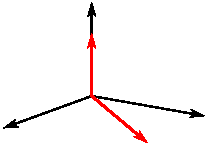
\includegraphics{images/HW02_1}}
    \put(10,-46){\small$x$} \put(44, 1){\small$z$} \put(103,-39){\small$y$}
    \put(56,-22){{\color{red}\small$\bfb$}} \put(62,-55){{\color{red}\small$\bfa$}}
  \end{picture}
%%%%%%%%%%%%%%%%%%%%%%%%%%%%%%%%%%%%%%%%%%%%%%%%%%%%%%%%%%%%%%%%%%%%%%%%%%%%%%%%%%%%%%%%%%%%%%%%%%%%

%%%%%%%%%%%%%%%%%%%%%%%%%%%%%%%%%%%%%%%%%%%%%%%%%%%%%%%%%%%%%%%%%%%%%%%%%%%%%%%%%%%%%%%%%%%%%%%%%%%%
\item Compute  the cross products $\langle 1,2,-3\rangle \times \langle 4,-7,5\rangle$
    \quad and \quad $(2\bfi + 3\bfj - 5\bfk)\times(-7\bfi +11\bfj + 13\bfk)$.
%%%%%%%%%%%%%%%%%%%%%%%%%%%%%%%%%%%%%%%%%%%%%%%%%%%%%%%%%%%%%%%%%%%%%%%%%%%%%%%%%%%%%%%%%%%%%%%%%%%%

%%%%%%%%%%%%%%%%%%%%%%%%%%%%%%%%%%%%%%%%%%%%%%%%%%%%%%%%%%%%%%%%%%%%%%%%%%%%%%%%%%%%%%%%%%%%%%%%%%%%
\item  Find a vector orthogonal to the plane of the three points, compute the area of the triangle they determine, and give an equation for
  the plane they lie on.\vspace{-5pt}
    \[  (0,2,4),\quad (-3,1,-5)\,,\quad (2,1,0)\,. \]
%%%%%%%%%%%%%%%%%%%%%%%%%%%%%%%%%%%%%%%%%%%%%%%%%%%%%%%%%%%%%%%%%%%%%%%%%%%%%%%%%%%%%%%%%%%%%%%%%%%%

%%%%%%%%%%%%%%%%%%%%%%%%%%%%%%%%%%%%%%%%%%%%%%%%%%%%%%%%%%%%%%%%%%%%%%%%%%%%%%%%%%%%%%%%%%%%%%%%%%%%
\item Prove the following formula for the vector triple product\vspace{-5pt}
  \[  \bfa\times(\bfb\times\bfc)\ =\ (\bfa\cdot\bfc)\bfb - (\bfa\cdot\bfb)\bfc\,. \]
%%%%%%%%%%%%%%%%%%%%%%%%%%%%%%%%%%%%%%%%%%%%%%%%%%%%%%%%%%%%%%%%%%%%%%%%%%%%%%%%%%%%%%%%%%%%%%%%%%%%

%%%%%%%%%%%%%%%%%%%%%%%%%%%%%%%%%%%%%%%%%%%%%%%%%%%%%%%%%%%%%%%%%%%%%%%%%%%%%%%%%%%%%%%%%%%%%%%%%%%%
\item Suppose that $\bfv_1$, $\bfv_2$, and $\bfv_3$ are vectors that are not coplanar.
  Define\vspace{-5pt}
   \[
   \bfk_1\ :=\ \frac{\bfv_2\times\bfv_3}{\bfv_1\cdot(\bfv_2\times\bfv_3)}\,, \qquad
   \bfk_2\ :=\ \frac{\bfv_3\times\bfv_1}{\bfv_1\cdot(\bfv_2\times\bfv_3)}\,, \quad \mbox{ and }\quad
   \bfk_3\ :=\ \frac{\bfv_1\times\bfv_2}{\bfv_1\cdot(\bfv_2\times\bfv_3)}\,.    \vspace{-5pt}
   \]
   (a) Show that if $i\neq j$, then $\bfk_i$ is orthogonal to $\bfv_j$.\newline
   (b) Show that $\bfk_i\cdot\bfv_i=1$ for $i=1,2,3$. \newline
   (c) Show that ${\displaystyle \bfk_1\cdot(\bfk_2\times\bfk_3)=\frac{1}{\bfv_1\cdot(\bfv_2\times\bfv_3)}}$.
   
%%%%%%%%%%%%%%%%%%%%%%%%%%%%%%%%%%%%%%%%%%%%%%%%%%%%%%%%%%%%%%%%%%%%%%%%%%%%%%%%%%%%%%%%%%%%%%%%%%%%




\end{enumerate}  
%%%%%%%%%%%%%%%%%%%%%%%%%%%%%%%%%%%%%%%%%%%%%%%%%%%%%%%%%%%%%%%%%%%%%%%%%%%%%%%%%%%%%%%%%%%%%%%%%%%%
\newpage

{\bf {\color{Maroon}Homework from section on equations for lines and planes.}}
%%%%%%%%%%%%%%%%%%%%%%%%%%%%%%%%%%%%%%%%%%%%%%%%%%%%%%%%%%%%%%%%%%%%%%%%%%%%%%%%%%%%%%%%%%%%%%%%%%%%
\begin{enumerate}  %  the \begin{..}  \end{..} stars and ends an environment.
\setcounter{enumi}{6}

%%%%%%%%%%%%%%%%%%%%%%%%%%%%%%%%%%%%%%%%%%%%%%%%%%%%%%%%%%%%%%%%%%%%%%%%%%%%%%%%%%%%%%%%%%%%%%%%%%%%
\item Give the vector and parametric equations for the line passing through the point $(-3,4,-5)$ and parallel to
  $\bfi -2\bfj +7\bfk$.
%%%%%%%%%%%%%%%%%%%%%%%%%%%%%%%%%%%%%%%%%%%%%%%%%%%%%%%%%%%%%%%%%%%%%%%%%%%%%%%%%%%%%%%%%%%%%%%%%%%%

%%%%%%%%%%%%%%%%%%%%%%%%%%%%%%%%%%%%%%%%%%%%%%%%%%%%%%%%%%%%%%%%%%%%%%%%%%%%%%%%%%%%%%%%%%%%%%%%%%%%
\item Show that the line through the points $(0,1,1)$ and $(1,-1,6)$ is perpendicular to the line  through the points 
  $(-4,2,1)$ and $(-1,6,2)$.
%%%%%%%%%%%%%%%%%%%%%%%%%%%%%%%%%%%%%%%%%%%%%%%%%%%%%%%%%%%%%%%%%%%%%%%%%%%%%%%%%%%%%%%%%%%%%%%%%%%%

%%%%%%%%%%%%%%%%%%%%%%%%%%%%%%%%%%%%%%%%%%%%%%%%%%%%%%%%%%%%%%%%%%%%%%%%%%%%%%%%%%%%%%%%%%%%%%%%%%%%
\item Determine whether the two lines are parallel, skew, or intersecting.  If they intersect, determine the point of
  intersection.\vspace{-5pt}
  \[
  L_1\colon x=1+t\,,\ y=2-t\,,\  z=1+3t\qquad
  L_2\colon x=2-s\,,\ y=1+2s\,,\ z=4+s\,.
  \]
%%%%%%%%%%%%%%%%%%%%%%%%%%%%%%%%%%%%%%%%%%%%%%%%%%%%%%%%%%%%%%%%%%%%%%%%%%%%%%%%%%%%%%%%%%%%%%%%%%%%

%%%%%%%%%%%%%%%%%%%%%%%%%%%%%%%%%%%%%%%%%%%%%%%%%%%%%%%%%%%%%%%%%%%%%%%%%%%%%%%%%%%%%%%%%%%%%%%%%%%%
\item Find the equation for the plane through $(-1,0,1)$ that contains the line $L_1$ of the previous exercise.
%%%%%%%%%%%%%%%%%%%%%%%%%%%%%%%%%%%%%%%%%%%%%%%%%%%%%%%%%%%%%%%%%%%%%%%%%%%%%%%%%%%%%%%%%%%%%%%%%%%%

%%%%%%%%%%%%%%%%%%%%%%%%%%%%%%%%%%%%%%%%%%%%%%%%%%%%%%%%%%%%%%%%%%%%%%%%%%%%%%%%%%%%%%%%%%%%%%%%%%%%
\item  Find the symmetric equation for the line of intersection of thetwo  planes with the given equations, as well as the angle between the
  planes\vspace{-5pt} 
  \[
  x-2y+z=2\quad\mbox{ and }\quad x+2y+z=1\,.
  \]
%%%%%%%%%%%%%%%%%%%%%%%%%%%%%%%%%%%%%%%%%%%%%%%%%%%%%%%%%%%%%%%%%%%%%%%%%%%%%%%%%%%%%%%%%%%%%%%%%%%%

%%%%%%%%%%%%%%%%%%%%%%%%%%%%%%%%%%%%%%%%%%%%%%%%%%%%%%%%%%%%%%%%%%%%%%%%%%%%%%%%%%%%%%%%%%%%%%%%%%%%
\item   Show that the lines $x=2+t$, $y=2-t$, $z=2t$ and  $x=-4+2s$, $y=1-s$, $z=3-s$ are skew, and determine the distance between them.  
%%%%%%%%%%%%%%%%%%%%%%%%%%%%%%%%%%%%%%%%%%%%%%%%%%%%%%%%%%%%%%%%%%%%%%%%%%%%%%%%%%%%%%%%%%%%%%%%%%%%

%%%%%%%%%%%%%%%%%%%%%%%%%%%%%%%%%%%%%%%%%%%%%%%%%%%%%%%%%%%%%%%%%%%%%%%%%%%%%%%%%%%%%%%%%%%%%%%%%%%%
\item  Find the parametric equation for the line through the point $(0,1,2)$ that is perpendicular to the line $x=1+t$,
  $y=1-t$, $z=2t$, and which intersects that line.
%%%%%%%%%%%%%%%%%%%%%%%%%%%%%%%%%%%%%%%%%%%%%%%%%%%%%%%%%%%%%%%%%%%%%%%%%%%%%%%%%%%%%%%%%%%%%%%%%%%%x

%%%%%%%%%%%%%%%%%%%%%%%%%%%%%%%%%%%%%%%%%%%%%%%%%%%%%%%%%%%%%%%%%%%%%%%%%%%%%%%%%%%%%%%%%%%%%%%%%%%%
\item   Find an equation for  the plane that contains the line of intersection of the two planes
  $x-z=1$ and $y+2z=3$, and which is also perpendicular to the plane $x+y-2z=4$.
%%%%%%%%%%%%%%%%%%%%%%%%%%%%%%%%%%%%%%%%%%%%%%%%%%%%%%%%%%%%%%%%%%%%%%%%%%%%%%%%%%%%%%%%%%%%%%%%%%%%



\end{enumerate}  
%%%%%%%%%%%%%%%%%%%%%%%%%%%%%%%%%%%%%%%%%%%%%%%%%%%%%%%%%%%%%%%%%%%%%%%%%%%%%%%%%%%%%%%%%%%%%%%%%%%%

\end{document}
